% Abstract file structure example : 
% \abstitle{title here}
% \absauthors{names and superscripts for affiliations here}
% \absaddress{affiliations, starting each one with its superscripts, separate affiliations with a \break}
% \abstext{
% \index{author abbreviated name, to be placed in authors' index}
% \index{create an index entry for each author}
%  The abstract text
% }

%% Abstract title
%\abstitle{Studio sui chirotteri troglofili della Grotta di Calafarina (Pachino, SR, Sicilia sud-orientale)}

%% Author names
%\absauthors{M. \textsc{Mucedda}$^1$,  G. \textsc{Fichera}$^2$, E. \textsc{Pidinchedda}$^1$}

%\absaddress{$^1$Centro Pipistrelli Sardegna, Via G. Leopardi 1 – 07100 Sassari, Italy - batsar@tiscali.it\break
%$^2$Universität Trier Universitätsring,15 - D-54286  Trier, Germany}

%% Abstract text
%\abstext{
%%% Author names for index. State each author separately using \index{Doe J.}
%\index{Mucedda M.}
%\index{Fichera G.}
%\index{Pidinchedda E.}
%%% The actual abstract text goes here
%} %% remember to close the abstract text block brace!!
\label{ext:E022}

\loadabstr[E022]{MUCEDDA M., PIDINCHEDDA E., BERTELLI M.L. -- Note sui pipistrelli nelle piccole isole della Sardegna}{abstracts/extended_abstracts/C022_mucedda.ea_extended_title.tex}

\begin{multicols}{2}

\section*{Introduzione}
Nell'arco di 20 anni è stata effettuata una indagine sul campo tendente a stabilire quali specie di pipistrelli siano presenti nelle piccole isole della Sardegna. Oggetto della ricerca sono state complessivamente 15 isole, a partire da nord: La Maddalena, Caprera, Santo Stefano, Spargi, Budelli, Santa Maria, Tavolara, Molara, Figarolo, Asinara, Piana, San Pietro, Sant’Antioco, Serpentara e Cavoli.

Sulle isole principali le ricerche sono state più approfondite e protratte a lungo negli anni, a partire dal 1994, mentre sulle isole minori le indagini sono state più ridotte, limitate talvolta ad una sola notte di monitoraggio.

\section*{Materiali e metodi}
Le indagini sono state condotte mediante esplorazione di rifugi, monitoraggio con \textit{bat detector} e raramente mediante catture notturne con le reti.

I rifugi sono stati individuati con l’esplorazione del territorio, localizzando strutture idonee ad ospitare pipistrelli, cioè edifici abbandonati, fortini militari, fessure nelle rocce, grotte naturali, cavità minerarie, gallerie artificiali. I controlli sono stati effettuati generalmente nelle ore diurne, quando i pipistrelli sono in fase di riposo, mediante osservazione diretta, facendo uso di lampade. Controlli sono stati eseguiti anche durante i movimenti notturni dei pipistrelli.

Poiché le isole minori sono praticamente prive di corsi d’acqua rilevanti, le poche catture sono state realizzate su vasconi o piccoli laghetti durante le attività di caccia notturna dei pipistrelli, utilizzando reti (\textit{mist-net}) specifiche per chirotteri sorrette da canne telescopiche. Gli animali catturati sono stati sottoposti alle principali misurazioni biometriche in vivo e liberati in breve tempo. Tutte le catture sono state effettuate con apposita autorizzazione del Ministero dell’Ambiente della Tutela del Territorio e del Mare. 

I monitoraggi notturni con \textit{bat detector} sono stati effettuati con quattro diversi strumenti: Pettersson D980, Pettersson D240x, Pettersson D1000 e Wildlife Acoustic Echo Meter EM3+, su punti fissi di registrazione lungo transetti in auto o a piedi.

Per l’analisi dei suoni e l’identificazione delle specie è stato utilizzato il software Batsound della Pettersson, utilizzando le metodiche di Barataud (2012) e tenendo conto dei valori riportati da Russo e Jones (2002).

\section*{Note bibliografiche}
I dati presenti in letteratura sui pipistrelli delle isole minori della Sardegna sono molto scarsi e riguardano solamente quattro isole. 

Zava e Violani (1992) riportano \emph{Myotis blythii}, \emph{Pipistrellus pipistrellus}, \emph{Pipistrellus kuhlii} e \emph{Tadarida teniotis} per l’Isola di San Pietro, segnalando anche un esemplare di \emph{Rhinolophus hipposideros} conservato nel Museo Zoologico Universitario di Torino. Riteniamo di non dover considerare valido il dato sul \emph{Myotis blythii}, in quanto nel territorio sardo questa specie non risulta presente.

Grafitti e Mucedda (1995) indicano la presenza di \emph{Rhinolophus ferrumequinum} e \emph{Miniopterus schreibersii} nell’Isola di Tavolara.

Zava et al. (1996) riportano le stesse informazioni pubblicate nel 1992 per l’Isola di San Pietro, cui aggiungono alcuni dati storici, segnalando per l'isola di La Maddalena un \emph{Pipistrellus kuhlii} conservato al Museo ``La Specola'' di Firenze (MZUF 13036) e per l'Isola di Sant'Antioco un \emph{Myotis myotis} conservato al Museo Civico di Storia Naturale di Milano (MSNM 722), risalente al 1912. Una nostra verifica effettuata presso quest’ultimo Museo ha consentito di stabilire che si tratta in realtà di \emph{Myotis punicus}, cui corrispondono le misurazioni biometriche (Giorgio Bardelli \textit{com. pers.}).

Mocci Demartis e Secci (1997) indicano \emph{Pipistrellus pipistrellus} per l’Isola di San Pietro.
Skiba (2009) segnala la registrazione di ultrasuoni di \emph{Myotis punicus} a Calasetta nell’Isola di Sant’Antioco.
Angelici et al. (2009) nella \textit{checklist} dei mammiferi delle piccole isole italiane riportano le indicazioni già citate dagli autori precedenti per San Pietro e La Maddalena. 

\begin{Figure} %[!ht]
  \centering\small
  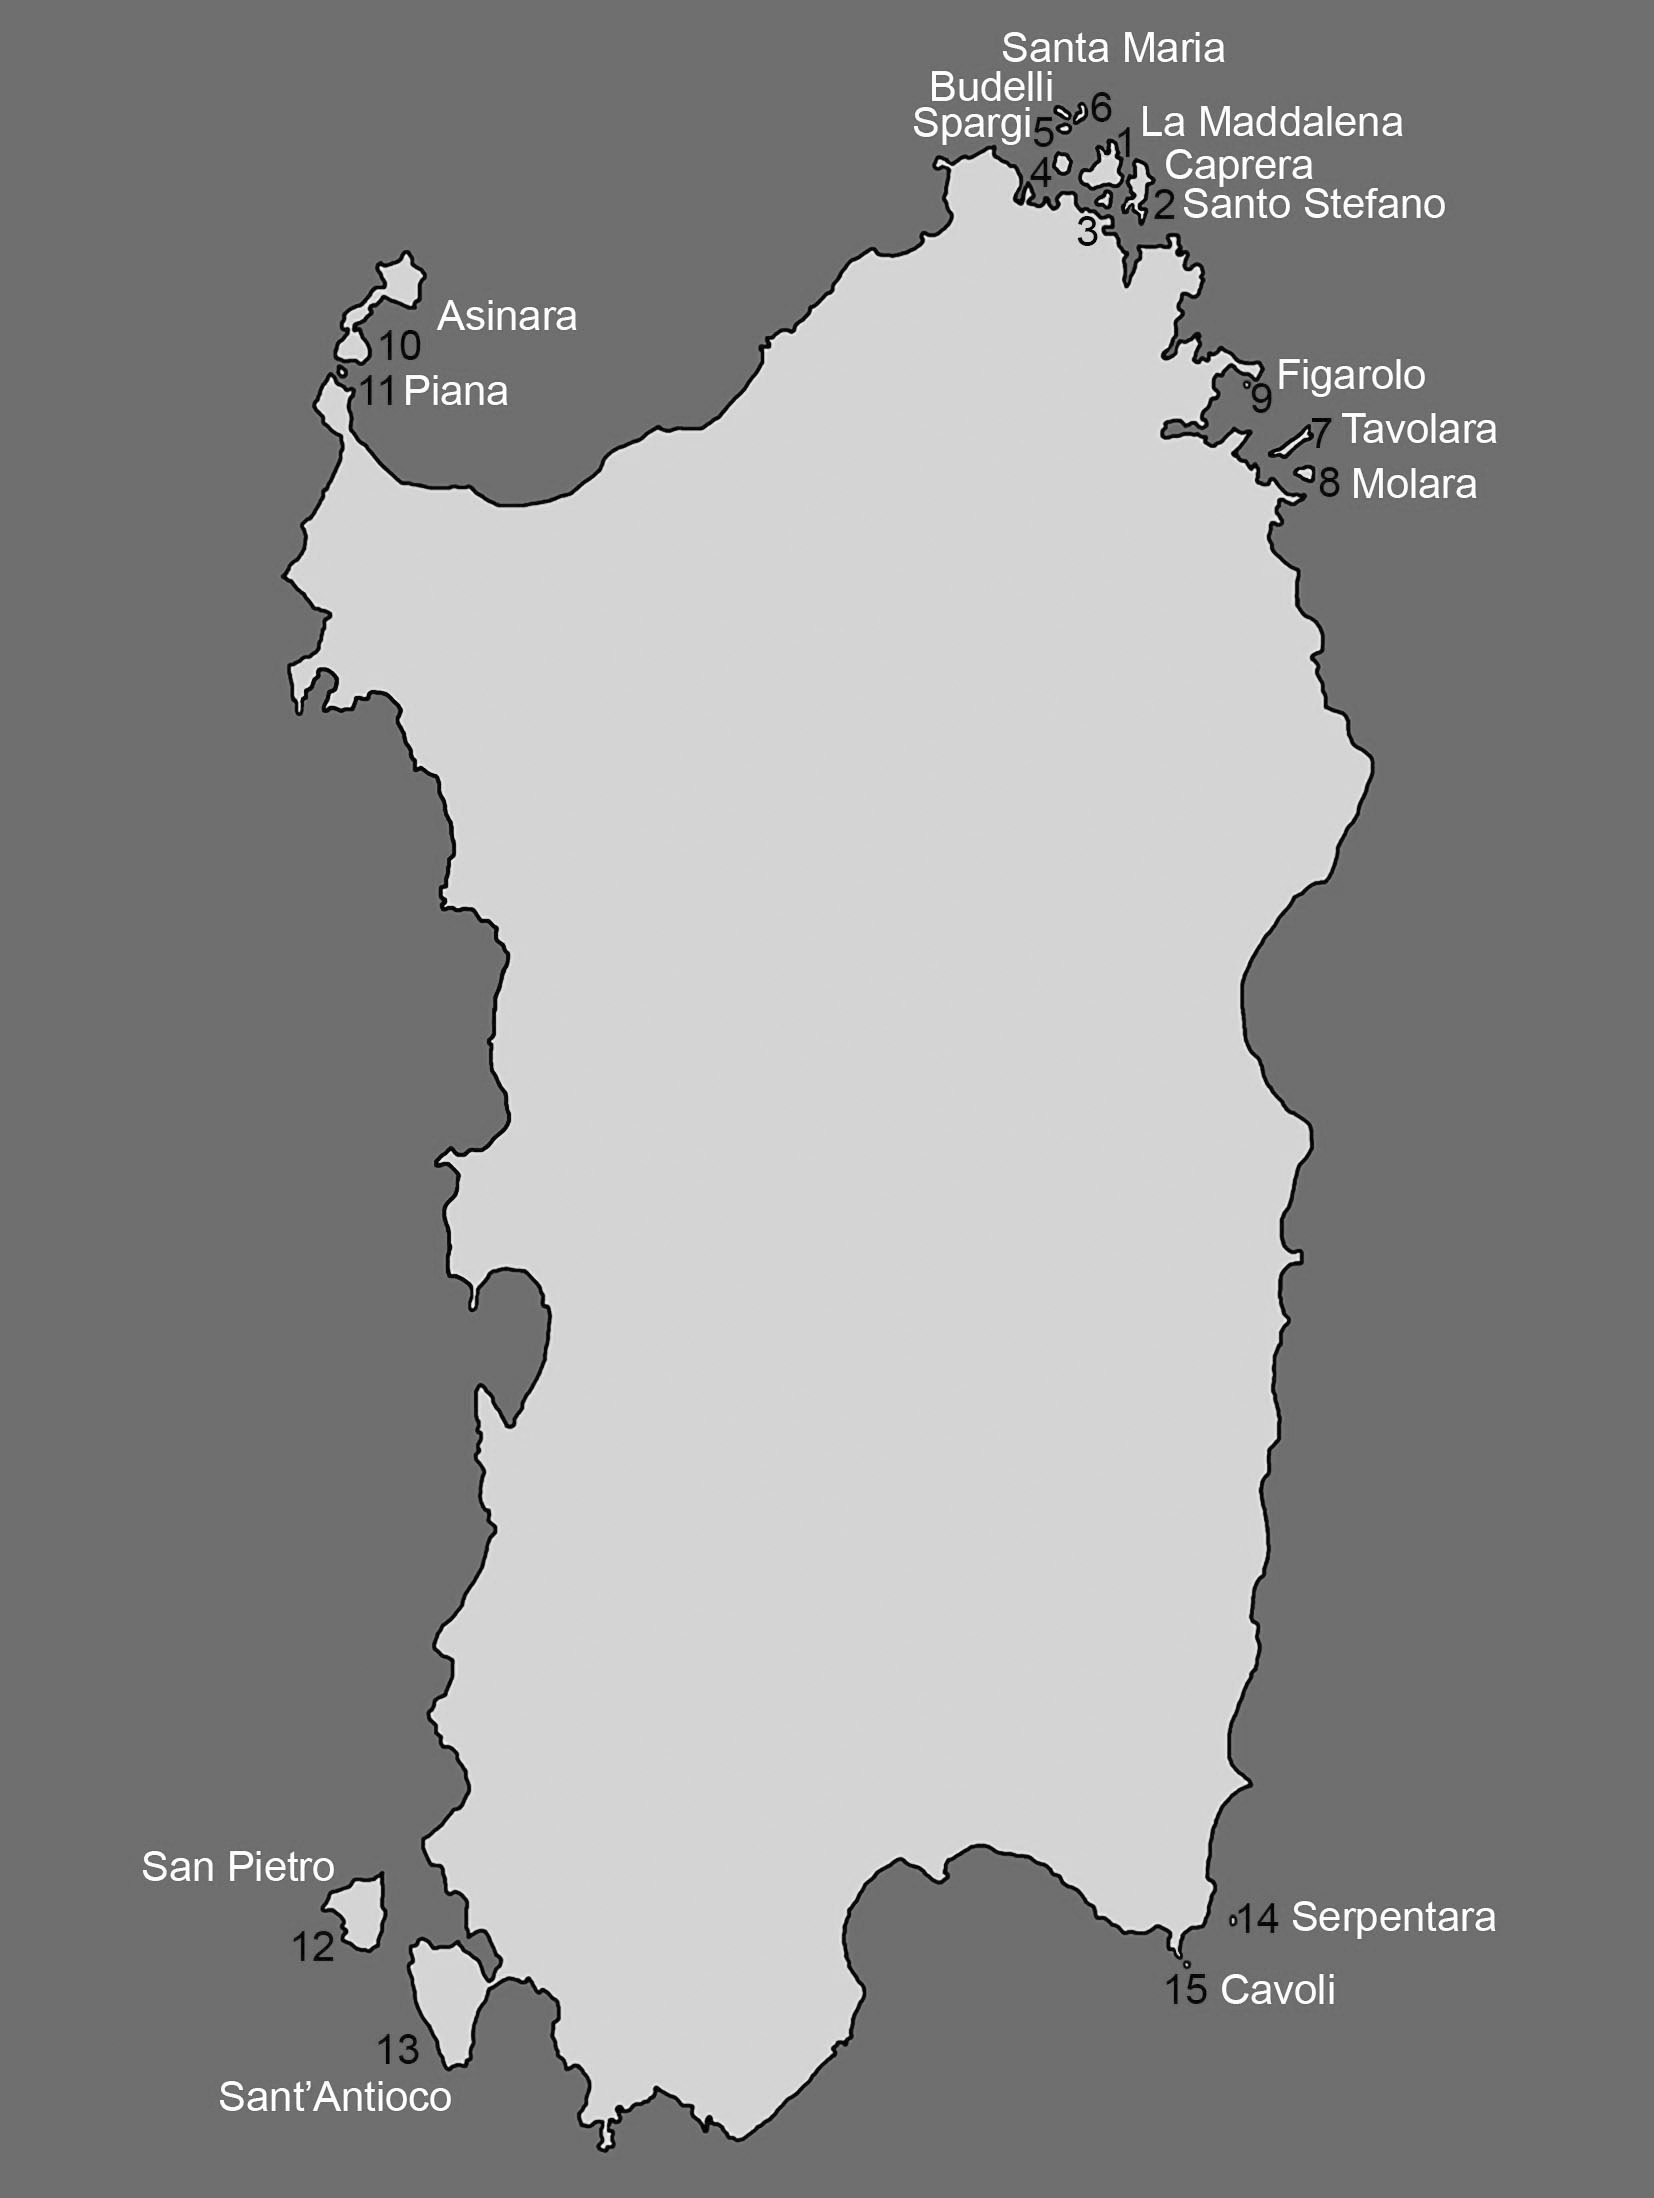
\includegraphics[width=\linewidth]{abstracts/extended_abstracts/C022_Figure1.png}
  \captionof*{}{Fig. 1 – Posizione geografica delle piccole isole della Sardegna.}
\end{Figure}

\section*{Risultati}
Riportiamo i risultati delle ricerche per ogni singola isola, a partire da nord verso sud.

\subsection*{Isola di La Maddalena (La Maddalena)}
È la principale isola dell’arcipelago, in cui ha sede la città di La Maddalena, con una popolazione di oltre 11000 abitanti. Ha una superficie di \SI{20.1}{\square\kilo\meter} e una quota massima di 212~m, ed è distante dalla costa sarda circa 2~km. Come tutte le isole dell’arcipelago è di natura granitica.

Le attività sono state effettuate in modo sporadico a partire dal 2005, e sono state completate con un monitoraggio della durata di un anno tra il 2010 e il 2011, finanziato dall’Ente Parco Nazionale dell’Arcipelago di La Maddalena. Le ricerche di rifugi di pipistrelli hanno interessato fortificazioni militari, edifici abbandonati, ruderi, civili abitazioni, gallerie, polveriere e riservette sotterranee, fessure nelle rocce.

Nell'Isola di La Maddalena sono stati localizzati 7 rifugi di pipistrelli, con la presenza di 4 specie.

Il monitoraggio col \textit{bat detector} è stato condotto in punti fissi di ascolto su un transetto in auto che si è svolto nelle strade sia lungo la cosa che nell’interno, compreso anche l'abitato.

In totale nell’isola, tra rifugi e monitoraggi notturni, è stata riscontrata la presenza di 7 specie di chirotteri:
\begin{compactdesc}
\item[\emph{Rhinolophus ferrumequinum}] osservato un solo esemplare in due diverse gallerie sotterranee, in letargo o riposo diurno.
\item[\emph{Myotis capaccinii}] pochi esemplari svernanti in una sola galleria sotterranea.
\item[\emph{Pipistrellus pipistrellus}] localizzato un rifugio con pochi esemplari in una galleria sotterranea e individuate quattro colonie in edifici, di cui solo due confermate come riproduttive; ampiamente contattato con il \textit{bat detector} ovunque nell’isola.
\item[\emph{Pipistrellus kuhlii}] ampiamente contattato con il \textit{bat detector} ovunque nell’isola.
\item[\emph{Hypsugo savii}], contattato con il \textit{bat detector} solo in poche località.
\item[\emph{Pipistrellus pygmaeus}/\emph{Miniopterus schreibersii}] pochi contatti registrati con il \textit{bat detector}, la cui analisi non ha consentito la discriminazione tra le due specie.
\item[\emph{Tadarida teniotis}] trovato un rifugio in una serie di fessure rocciose con almeno 35 individui osservati in uscita serale; contattato con il \textit{bat detector} nella parte occidentale dell’isola.
\end{compactdesc}

\subsection*{Isola di Caprera (La Maddalena - OL)}
È la seconda isola per importanza dell’arcipelago, con una superficie di \SI{15.7}{\square\kilo\meter} e una quota massima di 212~m. È collegata con un ponte a La Maddalena e ha una popolazione residente molto ridotta. 

Le attività sono state effettuate in modo sporadico a partire dal 2000, e sono state completate con un monitoraggio della durata di un anno tra il 2010 e il 2011, finanziato dall’Ente Parco Nazionale dell’Arcipelago di La Maddalena. Le ricerche di rifugi di pipistrelli hanno interessato fortificazioni militari, edifici abbandonati, ruderi, gallerie, polveriere e riservette sotterranee, fessure nelle rocce. 

Nell'Isola di Caprera sono stati individuati 14 rifugi di pipistrelli, con la presenza di 5 specie. Il monitoraggio col \textit{bat detector} è stato condotto in punti fissi di ascolto lungo tutte le strade dell’isola. 
In totale, tra rifugi e monitoraggi notturni, nell’Isola di Caprera è stata riscontrata la presenza di 8 specie.
\begin{compactdesc}
\item[\emph{Rhinolophus ferrumequinum}] osservato svernante o in riposo diurno, in numero di uno o due esemplari, in 7 gallerie sotterranee e 1 edificio.
\item[\emph{Rhinolophus hipposideros}] presente un solo esemplare in una struttura sotterranea militare.
\item[\emph{Myotis capaccinii}] osservato un solo esemplare in un vecchio edificio militare. 
\item[\emph{Pipistrellus pipistrellus}] osservato isolatamente in un rifugio sotterraneo e in tre edifici e catturato anche con le reti; è la specie più ampiamente contattata con il \textit{bat detector} ovunque nell’isola.
\item[\emph{Pipistrellus kuhlii}] contattato con il \textit{bat detector} in varie località.
\item[\emph{Hypsugo savii}] pochissimi contatti con il \textit{bat detector}.
\item[\emph{Pipistrellus pygmaeus}/\emph{Miniopterus schreibersii}] un solo contatto con il \textit{bat detector}.
\item[\emph{Tadarida teniotis}] presente una colonia di numero molto variabile in una fessura rocciosa, con max 38 esemplari conteggiati all’involo serale; contattato anche con il \textit{bat detector}.
\end{compactitem}

\subsection*{Isola di Santo Stefano (La Maddalena - OL)}
Ha una superficie di \SI{3}{\square\kilo\meter} e raggiunge la massima quota di 100~m. Distante 1~km dalla terraferma, l’isola non è disabitata, ma ha un insediamento turistico e una base militare.

Sono stati esplorati vari edifici abbandonati e una galleria sotterranea artificiale. Il monitoraggio col \textit{bat detector} è stato effettuato nell’agosto 2011 lungo un transetto a piedi sulle stradine dell’isola. 
In totale è stata riscontrata la presenza di 4 specie. 
\begin{compactdesc}
\item[\emph{Rhinolophus ferrumequinum}] osservato un solo esemplare in una galleria sotterranea.
\item[\emph{Pipistrellus pipistrellus}, \emph{Hypsugo savii} e \emph{Tadarida teniotis}] tutti con pochi contatti col \textit{bat detector} in diverse località.
\end{compactdesc}

\subsection*{Isola di Spargi (La Maddalena - OL)}
Con una superficie di \SI{4.2}{\square\kilo\meter} è la terza per estensione dell'Arcipelago, distante dalla costa 2.5~km. Raggiunge la quota massima di 153~m ed è normalmente disabitata, con qualche rara presenza umana limitata a soggiorno estivo.

Nell’Isola di Spargi le attività sono state svolte in maggio e in agosto 2011, con esplorazione di ruderi, vecchie strutture militari e una galleria sotterranea, in nessuna delle quali è stata riscontrata la presenza di pipistrelli.
Il monitoraggio col \textit{bat detector} è stato condotto con un transetto a piedi lungo i sentieri principali nella parte centrale e settentrionale dell’isola. Attività ridotta dei pipistrelli, con pochi contatti relativi a quattro specie registrate in diverse località: \emph{Pipistrellus pipistrellus}, \emph{Pipistrellus pygmaeus}/\emph{Miniopterus schreibersii}, \emph{Hypsugo savii} e \emph{Tadarida teniotis}.

\subsection*{Isola di Budelli (La Maddalena - OL)}
È distante circa 8~km dalla costa sarda, ha una superficie di \SI{1.6}{\square\kilo\meters} e si eleva sino alla quota di 88~m. Esiste una sola abitazione in cui vive il custode dell’isola.

Praticamente priva di potenziali rifugi, esplorate solamente due costruzioni e una fessura nella roccia.
Il monitoraggio col \textit{bat detector} è stato condotto nell’agosto 2011 lungo un transetto a piedi che ha interessato la parte orientale e centrale dell’isola. Pochi i contatti di pipistrelli, relativi a due sole specie in differenti località: \emph{Pipistrellus pipistrellus} più frequente e \emph{Tadarida teniotis}.

\subsection*{Isola di Santa Maria (La Maddalena - OL)}
È la più lontana dalla costa sarda, da cui dista 9~km, ha una superficie di \SI{2}{\square\kilo\meter} ed è la più bassa delle isole dell’arcipelago con una quota massima di soli 49 metri.

Sull’isola esistono una struttura alberghiera e poche abitazioni, utilizzate per lo più in periodo estivo.
Le ricerche di rifugi hanno interessato solamente 4 strutture edilizie, in nessuna delle quali è stata riscontrata la presenza di pipistrelli.

Il monitoraggio col \textit{bat detector} è stato realizzato nel luglio 2011 lungo un transetto a piedi nei sentieri che percorrono l’isola longitudinalmente. La registrazione dei suoni ha consentito di accertare la presenza di una sola specie di pipistrello: \emph{Pipistrellus pipistrellus}, contattata in diverse località.

\subsection*{Isola di Tavolara (Olbia - OL)}
Costituita da una basamento granitico, su cui si poggia un’imponente copertura calcarea mesozoica, che si eleva con carattere di montagna sino a 565~m di quota, la più alta di tutte le isole circumsarde. Situata a circa 2~km dalla costa, ha una superficie di \SI{5.9}{\square\kilo\meter}. Nella sua estremità di NE è sede di una base militare, mentre nella parte SO vi si trovano alcune case e alcune strutture di tipo turistico attive solo in periodo estivo.

Le prime ricerche sono state effettuate nel 1994 (Grafitti \& Mucedda, 1995) e sono riprese successivamente negli anni 2009-2013. Sono state esplorate alcune grotte ed edifici e sono stati effettuati tre monitoraggi notturni col \textit{bat detector} lungo transetti a piedi nell’unica stradina e sui sentieri nella sola parte SO non militarizzata dell’isola.
È stata riscontrata la presenza di 8 specie di pipistrelli. 
\begin{compactdesc}
\item[\emph{Rhinolophus ferrumequinum}] presente con un solo esemplare nella grotta Inghiottitoio della Mandria e nella vicina Grotta Findema.
\item[\emph{Miniopterus schreibersii}] osservati una decina di esemplari nella Grotta dei Fiori d’Arancio.
\item[\emph{Pipistrellus pipistrellus} e \emph{Pipistrellus kuhlii}] sono le specie più frequentemente contattate con il \textit{bat detector} in varie località, anche sulla spiaggia.
\item[\emph{Hypsugo savii} e \emph{Tadarida teniotis}] contattate con il \textit{bat detector}, meno frequenti delle due specie precedenti. 
\item[\emph{Myotis} indet.] un solo contatto che non ha consentito di identificare la specie.
\item[\emph{Eptesicus serotinus}] contattato ripetutamente in caccia su un’area pinetata. Si ritiene valida l’identificazione grazie a numerose registrazioni in successione, in cui non si evidenzia mai alternanza delle due tipologie di segnali, escludendo così che si possa trattare di \emph{Nyctalus leisleri} con cui può essere facilmente confuso.
\end{compactdesc}

\subsection*{Isola di Molara (Olbia - OL)}
Di natura granitica, ha una superficie di \SI{3.4}{\square\kilo\meter} e raggiunge la massima quota di 155~m. È distante dalla costa circa 2~km ed è disabitata.

Le ricerche si sono svolte con il controllo di alcuni edifici, che non hanno rivelato tracce di pipistrelli, e con una sola notte di registrazioni col \textit{bat detector}, lungo un transetto a piedi sui sentieri, nell’agosto 2012. È stata riscontrata la presenza di 3 specie: 
\begin{compactdesc}
\item[\emph{Pipistrellus pipistrellus}] ampiamente presente in tutta l’isola. 
\item[\emph{Hypsugo savii}] un solo contatto nella parte sommitale dell’isola.
\item[\emph{Tadarida teniotis}] registrato in diverse località.
\end{compactdesc}

\subsection*{Isola di Figarolo (Golfo Aranci - OL)}
Minuscola isoletta disabitata, con una superficie di \SI{0.2}{\square\kilo\meter}, la più piccola tra quelle visitate, situata a soli 350~m dalla costa. Geologicamente ha un basamento granitico sul quale poggiano delle bancate calcaree dell’era Mesozoica, con vegetazione a macchia mediterranea e fitte aree boscate, che raggiunge la massima quota di 139~m.
  
Le ricerche hanno interessato una sola notte di registrazioni col \textit{bat detector}, lungo un transetto a piedi, nell’agosto 2014.
Nonostante le sue ridotte dimensioni vi è stata riscontrata la presenza di 4 specie: \emph{Pipistrellus pipistrellus}, \emph{Pipistrellus kuhlii}, \emph{Hypsugo savii} e \emph{Tadarida teniotis}, tutte con contatti poco numerosi.

\subsection*{Isola dell'Asinara (Porto Torres - SS)}
Costituisce un Parco Nazionale, con una superficie di \SI{51}{\square\kilo\meter} e non ha una popolazione residente, ma solo attività legate alla valorizzazione turistica e alla tutela ambientale. Di natura granitica e scistosa, raggiunge la massima altitudine di 408~m.

Nell’Isola dell’Asinara sono state effettuate ricerche saltuarie a partire dal 1995, proseguite poi in modo più approfondito dal 2008 al 2015.
Le ricerche si sono basate sulla individuazione dei rifugi di pipistrelli, catture con le reti e registrazioni notturne col \textit{bat detector}. Negli ultimi anni le attività sono state condotte in collaborazione con Rebecca Winter, che ha svolto sull’isola intense indagini triennali per il suo Dottorato presso l’Università di Hildesheim in Germania. 

Sono stati localizzati 30 rifugi in edifici e altre strutture e 2 in piccole cavità sotterranee artificiali. 
In totale sono state individuate 10 specie di pipistrelli: 
\begin{compactdesc}
\item[\emph{Rhinolophus ferrumequinum}] osservato in numero molto ridotto di esemplari in edifici e in cavità sotterranee artificiali, per un totale di 10 rifugi.
\item[\emph{Rhinolophus hipposideros}] è la specie più numerosa negli edifici abbandonati, osservata anche in cisterne. Individuati 11 rifugi e 2 colonie di riproduzione, con un massimo di circa 40 esemplari presenti. Contattato anche con il \textit{bat detector}.
\item[\emph{Myotis daubentonii}] osservato in tutti i laghetti presenti sull’isola e catturato con le reti in pochi esemplari. 
\item[\emph{Miniopterus schreibersii}] catturato un solo esemplare con le reti. 
\item[\emph{Pipistrellus pipistrellus}] è la specie più ampiamente contattata con il \textit{bat detector} ovunque nell’isola. Utilizza anche edifici, con piccole colonie che si annidano generalmente dietro le grondaie. Catturato anche con le reti.
\item[\emph{Pipistrellus kuhlii}] è la seconda specie più ampiamente contattata con il \textit{bat detector}, catturato anche con le reti. 
\item[\emph{Pipistrellus pygmaeus}] pochi contatti con il \textit{bat detector}, identificato dall’analisi dei \textit{social calls}. 
\item[\emph{Hypsugo savii}] pochissimi contatti con il \textit{bat detector}. 
\item[\emph{Eptesicus serotinus} o \emph{Nyctalus leisleri}] pochissimi contatti con il \textit{bat detector}. Dai soli suoni registrati non è stato possibile discriminare tra le due specie.
\item[\emph{Tadarida teniotis}] contattato con il \textit{bat detector} in varie parti dell’isola. 
\end{compactdesc}

\subsection*{Isola Piana (Porto Torres - SS)}
Piccola isoletta che ha una superficie di \SI{1.4}{\square\kilo\meter}, è situata a 600~m dalla costa ed è disabitata. È di natura scistosa, con bassa e rada vegetazione a macchia mediterranea, che si eleva solo sino a 24 di quota. 

Le ricerche sono state effettuate per una sola notte nell’agosto 2015. Controllata la Torre spagnola, l’unica struttura edilizia presente che è risultata priva di pipistrelli.
L’attività notturna dei pipistrelli si è rivelata inizialmente abbondante su una piccola polla d’acqua nella parte nord dell’isola, poi scarsa con pochi contatti al \textit{bat detector}.
Lungo un transetto a piedi che ha interessato quasi tutta l’isola è stata rilevata la presenza di due sole specie: \emph{Pipistrellus pipistrellus} più frequente e \emph{Pipistrellus kuhlii} meno frequente. 

\subsection*{Isola di San Pietro (Carloforte - CI)}
È un’isola di natura vulcanica di \SI{51}{\square\kilo\meter} di superficie ed è abitata, con la cittadina di Carloforte che ha circa 6500 abitanti. È distante circa 7~km dalla costa sarda e ha la massima altitudine di 211~m.

Nell’Isola di San Pietro le nostre attività hanno avuto inizio nel 1995 e si sono protratte in modo saltuario sino al 2013. Le ricerche si sono articolate con l’individuazione di rifugi di pipistrelli e registrazioni notturne col \textit{bat detector}, lungo transetti in auto che hanno interessato tutta l’isola.
È stata accertata la presenza di 5 specie di pipistrelli: 
\begin{compactdesc}
\item[\emph{Rhinolophus hipposideros}] è stato osservato in due gallerie minerarie e registrato in attività notturna col \textit{bat detector}. 
\item[\emph{Myotis capaccinii}] presenti piccoli gruppi di qualche decina di esemplari in una galleria mineraria. 
\item[\emph{Pipistrellus pipistrellus}] è la specie più ampiamente contattata con il \textit{bat detector} in tutta nell’isola. 
\item[\emph{Pipistrellus kuhlii}] pochi contatti con il \textit{bat detector}. 
\item[\emph{Tadarida teniotis}] contattata con il \textit{bat detector} in varie parti dell’isola. 
\end{compactdesc}

\subsection*{Isola di Sant'Antioco (Sant'Antioco e Calasetta – CI)}
Sant'Antioco con una superficie di \SI{108.9}{\square\kilo\meter} è una delle maggiori isole italiane, con due centri abitati, Sant’Antioco e Calasetta, e una popolazione totale di oltre 14000 abitanti. È collegata alla terraferma con un istmo e un ponte, è di natura prevalentemente vulcanica con ridotti lembi calcarei e raggiunge la massima quota di 273~m.

Le attività sono state effettuate negli anni 2002, 2006, 2010 e 2014. Le ricerche di rifugi di pipistrelli hanno interessato alcune grotte, edifici abbandonati, la necropoli punica. Le catture con le reti sono state effettuate in una sola occasione in un laghetto. Le registrazioni notturne con \textit{bat detector} sono state realizzate lungo transetti in auto in tre diverse occasioni e hanno interessato quasi tutta l’isola.
In totale è stata accertata la presenza a Sant’Antioco di 6 specie di chirotteri: 
\begin{compactdesc}
\item[\emph{Rhinolophus hipposideros}] è stato osservato isolatamente in due sole cavità sotterranee, una tomba della Necropli Punica e la Grotta di Sargaltas. 
\item[\emph{Miniopterus schreibersii}] un solo esemplare rinvenuto all’esterno di un edificio nel centro abitato di Sant’Antioco.
\item[\emph{Pipistrellus pipistrellus}] contattato con \textit{bat detector} ovunque nell’isola, catturato anche con le reti. 
\item[\emph{Pipistrellus kuhlii}] contattato con il \textit{bat detector} meno frequentemente della specie precedente. 
\item[\emph{Hypsugo savii}] contattato con il \textit{bat detector} in poche località. 
\item[\emph{Tadarida teniotis}] contattato con il \textit{bat detector} solo in poche occasioni. 
\end{compactdesc}
A questo elenco si deve aggiungere il \emph{Myotis punicus}, già citato da Zava et Al. (1996) e segnalato anche da Skiba (2009), di cui noi non abbiamo accertato la presenza attuale sull’isola.

\subsection*{Isola di Serpentara (Villasimius – CA)}
È un’isola molto piccola, con una superficie di solo \SI{1.34}{\square\kilo\meter}, che raggiunge la massima quota di 54~m e dista poco più di 3~km dalla costa sarda. È di natura granitica, con vegetazione a macchia mediterranea ed è disabitata. 

Le ricerche sono state effettuate per una sola giornata e una notte nell’agosto 2013. Controllate la torre spagnola, unico edificio presente, e piccole cavità e tafoni; non è stato individuato alcun rifugio di pipistrelli né tracce della loro presenza.
Lungo un transetto a piedi che ha interessato quasi tutta l’isola è stata rilevata la presenza di due sole specie: \emph{Pipistrellus pipistrellus} e \emph{Tadarida teniotis}.

\begin{table*}[t]
\caption*{Tab. 1 - Elenco delle specie rilevate per ciascuna delle isole monitorate. N\degree{}: numero di specie rilevate. L'ultima riga indica il numero di isole su cui è stata rilevataciascuna specie. Rfe=\emph{Rhinolophus ferrumequinum}; Rhi=\emph{Rhinolophus hipposideros}; Mca=\emph{Myotis capaccinii}; Mda=\emph{Myotis daubentonii}; Myo=\emph{Myotis} sp.; Msc=\emph{Miniopterus schreibersii}; Ppi=\emph{Pipistrellus pipistrellus}; Pku=\emph{Pipistrellus kuhlii}; Hsa=\emph{Hypsugo savii}; Ppyg=\emph{Pipistrellus pygmaeus}; Ese=\emph{Eptesicus serotinus}; Tte=\emph{Tadarida teniotis}.}
%\label{tab:table1}
\centering\small
\begin{tabular}{lccccccccccccc}
\quad & \textbf{N\degree{}} & \textbf{Rfe} & \textbf{Rhi} & \textbf{Mca} & \textbf{Mda} & \textbf{Myo} & \textbf{Msc} & \textbf{Ppi} & \textbf{Pku} & \textbf{Ppyg} & \textbf{Hsa} & \textbf{Ese} & \textbf{Tte} \\
\hline
La Maddalena  &  7 & $\times$ &          & $\times$ &          &          &          & $\times$ & $\times$ & $\times$? & $\times$ &           & $\times$ \\
Caprera       &  8 & $\times$ & $\times$ & $\times$ &          &          &          & $\times$ & $\times$ & $\times$? & $\times$ &           & $\times$ \\
Santo Stefano &  4 & $\times$ &          &          &          &          &          & $\times$ &          &           & $\times$ &           & $\times$ \\
Spargi        &  2 &          &          &          &          &          &          & $\times$ &          & $\times$? & $\times$ &           & $\times$ \\
Budelli       &  2 &          &          &          &          &          &          & $\times$ &          &           &          &           & $\times$ \\
Santa Maria   &  1 &          &          &          &          &          &          & $\times$ &          &           &          &           &          \\
Tavolara      &  8 & $\times$ &          &          &          & $\times$ & $\times$ & $\times$ & $\times$ &           & $\times$ & $\times$  & $\times$ \\
Molara        &  3 &          &          &          &          &          &          & $\times$ &          &           & $\times$ &           & $\times$ \\
Figarolo      &  4 &          &          &          &          &          &          & $\times$ & $\times$ &           & $\times$ &           & $\times$ \\
Asinara       & 10 & $\times$ & $\times$ &          & $\times$ &          & $\times$ & $\times$ & $\times$ & $\times$  & $\times$ & $\times$? & $\times$ \\
Piana         &  2 &          &          &          &          &          &          & $\times$ & $\times$ &           &          &           &          \\
San Pietro    &  5 &          & $\times$ & $\times$ &          &          &          & $\times$ & $\times$ &           &          &           & $\times$ \\
Sant’Antioco  &  6 &          & $\times$ &          &          &          & $\times$ & $\times$ & $\times$ &           & $\times$ &           & $\times$ \\
Serpentara    &  2 &          &          &          &          &          &          & $\times$ &          &           &          &           & $\times$ \\
Cavoli        &  2 &          &          &          &          &          &          & $\times$ & $\times$ &           &          &           &          \\
N\degree{} isole &    &        5 &        4 &        3 &        1 &        1 &        3 &       15 &        9 &         4 &        9 &         2 &       12 \\
\end{tabular}
\end{table*}

\subsection*{Isola dei Cavoli (Villasimius – CA)}
Minuscola isola con una superficie di \SI{0.43}{\square\kilo\meter}, è distante solo 700~m dalla estrema punta sud orientale della Sardegna ed è disabitata. È di natura granitica, con bassa vegetazione a macchia mediterranea, e raggiunge solo la quota di 40~m.
 
Le ricerche sono state effettuate per una sola giornata e una notte nel luglio 2012. Nelle due uniche strutture edilizie presenti non è stato individuato alcun rifugio di pipistrelli.
Lungo un transetto a piedi che ha interessato tutta l’isola sono stati registrati pochissimi contatti che hanno rivelato la presenza di due sole specie: \emph{Pipistrellus pipistrellus} e \emph{Pipistrellus kuhlii}.

A queste 15 si devono aggiungere l’Isola di Razzoli e l’isolotto del Porco nell’Arcipelago di La Maddalena e l’isolotto della Foradada nel comune di Alghero, in cui sono state fatte solo prospezioni diurne che non hanno rivelato la presenza di pipistrelli.

\section*{Discussione}
Su 21 specie di chirotteri presenti nella Sardegna, almeno 11 sono state riscontrate nel totale delle isole minori.
\begin{compactitem}
\item Rinolofo maggiore (\emph{Rhinolophus ferrumequinum} Schreber, 1774)
\item Rinolofo minore (\emph{Rhinolophus hipposideros} Bechstein, 1800)
\item Vespertilio di Capaccini (\emph{Myotis capaccinii} Bonaparte, 1837)
\item Vespertilio di Daubenton (\emph{Myotis daubentonii} Kuhl, 1819)
\item Pipistrello nano (\emph{Pipistrellus pipistrellus} Schreber, 1774)
\item Pipistrello albolimbato (\emph{Pipistrellus kuhlii} Kuhl, 1817)
\item Pipistrello pigmeo (\emph{Pipistrellus pygmaeus} Leach, 1825)
\item Pipistrello di Savi (\emph{Hypsugo savii} Bonaparte, 1837)
\item Serotino comune (\emph{Eptesicus serotinus} Schreber, 1774) o Nottola di Leisler (\emph{Nyctalus leisleri} Kuhl, 1818)
\item Miniottero (\emph{Miniopterus schreibersii} Kuhl, 1817)
\item Molosso di Cestoni (\emph{Tadarida teniotis} Rafinesque, 1814)
\end{compactitem}

Tra le specie contattate solamente col \textit{bat detector}, alcune non è stato possibile identificarle con certezza. È il caso della coppia \emph{Pipistrellus pygmaeus}---\emph{Miniopterus schreibersii} per l’Arcipelago di La Maddalena e \emph{Eptesicus serotinus}---\emph{Nyctalus leisleri} per l’Asinara, considerate come un’unica entità in quanto non è stato possibile distinguerle sulla base delle loro emissioni ultrasonore, per cui nel conteggio delle specie si intende presente l’una o l’altra delle due. Il \emph{Pipistrellus pygmaeus} all’Asinara è stato invece identificato con certezza sulla base dei \textit{social calls}. 

Come già detto in precedenza, si ritiene valida anche l’identificazione di \emph{Eptesicus serotinus} a Tavolara, le cui registrazioni non evidenziano mai alternanza delle due tipologie di segnali.

Nella Tab. 1 si riportano per ognuna delle 15 isole monitorate, da nord a sud, le specie di pipistrelli da noi riscontrate come presenti. 

La seconda colonna della Tab. 1 (N\degree{}) mostra il numero di specie presenti in ogni singola isola; l’ultima riga indica il numero di isole in cui è presente ogni singola specie.

Il più alto numero di specie si riscontra all’Asinara con 10 entità, seguita da Caprera e Tavolara con 8, quindi La Maddalena con 7. Nelle altre isole il numero va a diminuire, riducendosi notevolmente nelle isolette più piccole sino al minimo di una sola specie.

In un’ampia visione che riguarda tutta l’Italia, sulla base di quanto pubblicato da Angelici et al. (2009), l’Asinara (10 specie) detiene il più elevato numero di entità alla pari con l’Isola d’Elba, Caprera e Tavolara (8 specie) superano l’Isola del Giglio (7 specie) che è alla pari con La Maddalena. Come particolarità, nelle isole sarde compaiono \emph{Myotis capaccinii}, \emph{Myotis daubentonii} e \emph{Pipistrellus pygmaeus} che non risultano sinora presenti in altre piccole isole italiane.

Le specie più ampiamente diffuse sono \emph{Pipistrellus pipistrellus}, presente in tutte le isole, seguita da \emph{Tadarida teniotis} in 12 isole, \emph{Hypsugo savii} e \emph{Pipistrellus kuhlii} in 9 isole. La più rara è risultata invece \emph{Myotis daubentonii} presente solo all’Asinara.

La specie troglofila più diffusa è \emph{Rhinolophus ferrumequinum}, presente in 5 isole.

Facendo un ulteriore confronto con le altre 26 isole italiane citate in Angelici et al. (2009), a differenza di quelle sarde in ambito italiano il più diffuso è \emph{Pipistrellus kuhlii} presente in 20 isole, mentre \emph{Pipistrellus pipistrellus} è presente in sole 11 isole, seguito da \emph{Tadarida teniotis} in 10 isole. 

Dal nostro studio emerge che la maggior parte dei contatti con i chirotteri nelle isole circumsarde avviene mediante l’uso del \textit{bat detector}. Se andiamo a valutare la somma delle specie contattate nella totalità delle isole, emerge infatti che su un valore cumulato di 68 identificazioni di specie, quelle contattate solo con \textit{bat detector} ammontano a 43, mentre quelle identificate mediante osservazione diretta nei rifugi o cattura sono 19 e quelle identificate con entrambi i metodi sono 6. Si sottolinea pertanto l’importanza crescente del metodo di identificazione bioacustica nei monitoraggi della chirotterofauna, anche se non sempre si può giungere ad una identificazione certa delle specie contattate.

Le isole oggetto dello studio ricadono tutte all’interno di aree protette. Più esattamente La Maddalena, Caprera, Santo Stefano, Spargi, Budelli e Santa Maria sono all’interno del Parco Nazionale dell’Arcipelago di La Maddalena; Tavolara e Molara ricadono nell’Area Marina Protetta Tavolara-Capo Coda Cavallo; Figarolo appartiene al Sito di Interesse Comunitario di Capo Figari; Asinara è Parco Nazionale, area SIC e ZPS; Piana è compresa nell’area SIC dell’Asinara; San Pietro è interamente Sito di Interesse Comunitario; Sant’Antioco presenta varie aree SIC che interessano parzialmente il suo territorio; Serpentara e Cavoli ricadono entrambe nell’Area Marina Protetta di Capo Carbonara.

\vskip3mm

\begin{small}
\noindent\textbf{Ringraziamenti}\\
Le ricerche sulle isole si sono avvalse della collaborazione preziosa di un gran numero di persone ed Enti che qui ringraziamo riportandoli in ordine sparso. Parco Nazionale dell’Arcipelago di La Maddalena, Antonella Gaio, Luca Bittau, Valentina Gilioli, Gaetano Pedroni, Alessandro Ragni, Mauro Morandi, Tommaso Gamboni, Irene Galante, Francesco Muzzu, Laura Aversano, Paolo Agnelli, Giuseppe Are, Parco Nazionale dell’Asinara, Pierpaolo Congiatu, Giovanni Careddu, Giuseppe Grieco, Danilo Pisu, Cristina Fiesoli, Angelo Pittalis, Veronica Pisu, Antonio Guiso, Stefania Piras, Simone Rosa, Giuliana Atzori, Anna Laura Tanca, Rebecca Winter, Julia Treitler, Tim Drissen, Robin Stadtmann, Area Marina Protetta di Tavolara e Capo Coda Cavallo, Giovanna Spano, Massimo Putzu, Diego Gaia, Area Marina Protetta di Capo Carbonara, Bruno Paliaga, Fabrizio Atzori, Soprintendenza Archeologica di Cagliari, Luciano Durante, Sandro Mezzolani, Francesco Livretti, Marco Siddi, Giorgio Bardelli, Gaetano Fichera, Luca Montanaro, Enrico Melis, Alessio Sale. 

\vskip3mm

\noindent\textbf{Bibliografia}\\

Angelici F.M., Laurenti A., Nappi A., 2009. A checklist of the mammals of small italian islands. Hystrix 20(1): 3--27.

Barataud M., 2012. Ecologie acoustique des chiropteres d’Europe. Biotope editions: 343 pp.

Grafitti G., Mucedda M., 1995. Le grotte dell'Isola di Tavolara e la loro fauna. Biogeographia XVIII: 51--62.

Mocci Demartis A., Secci A., 1997. Dati sulla distribuzione dei Chirotteri nella Sardegna meridionale. Rend. Sem. Fac. Scienze Univ. Di Cagliari, 67: 61--74.

Russo D, Jones G., 2002. Identification of twenty-two bat species (Mammalia: Chiroptera) from Italy by analysis of time-expanded recordings of echolocation calls. J. Zool., London, 258: 91--103.

Skiba R., 2009. Europäische Fledermäuse. Westarp Wissenschaften: 128.

Zava B., Fiore M., Fornasari L., Violani C., 1996. Note sui Chirotteri dell'Isola di San Pietro con cenni storici sulle ricerche chirotterologiche in Sardegna. Biogeographia, XVIII: 641--651.

Zava B., Violani C., 1992. Nuovi dati sulla chirotterofauna italiana. Boll. Mus. Reg. Sci. Nat. Torino, 10 (2): 261-264.

\end{small}

\end{multicols}
% % EOF % %